\begin{figure}
	\begin{center}
		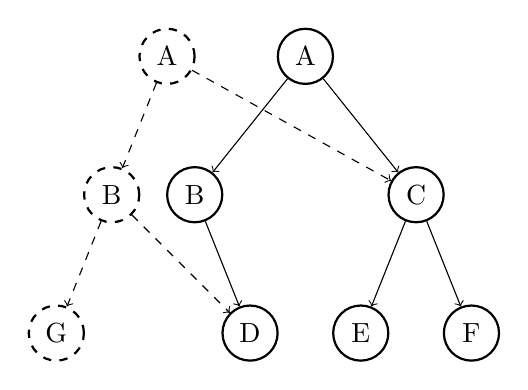
\begin{tikzpicture}[
			oldnode/.style={circle, draw=black, thick, minimum size=7mm},
			newnode/.style={circle, thick, draw=black, dashed, minimum size=7mm},
			]
			\node[oldnode] at (0,0) (root) {A};
			\node[oldnode] at (-4em,-5em) (beta) {B};
			\node[oldnode] at (4em,-5em) (gamma) {C};
			\node[oldnode] at (-2em,-10em) (delta) {D};
			\node[oldnode] at (2em,-10em) (epsilon) {E};
			\node[oldnode] at (6em,-10em) (zeta) {F};
			\node[newnode] at (-5em,0) (newroot) {A};
			\node[newnode] at (-7em,-5em) (newbeta) {B};
			\node[newnode] at (-9em,-10em) (newvertex) {G};
			\draw[->] (root) -- (beta);
			\draw[->] (root) -- (gamma);
			\draw[->] (beta) -- (delta);
			\draw[->] (gamma) -- (zeta);
			\draw[->] (gamma) -- (epsilon);
			\draw[->,dashed] (newroot) -- (gamma);
			\draw[->,dashed] (newroot) -- (newbeta);
			\draw[->,dashed] (newbeta) -- (newvertex);
			\draw[->,dashed] (newbeta) -- (delta);
		\end{tikzpicture}
	\end{center}
	{
		\small
		A new vertex G was added to the structure with solid vertices. 
		Dashed vertices were created by the update -- path from G to the root. 
		Dashed A is the new root.
	}
	\caption{Path-copying}
	\label{fig:path-copying}
\end{figure}